\documentclass[../main/main.tex]{subfiles}

\newdate{date}{06}{05}{2020}

\begin{document}

\section{Lecture 17}
 \displaydate{date}. Compiled:  \today. Alessandra+Alice.

\subsubsection{Slide 274}

\begin{figure}[h!]
\centering
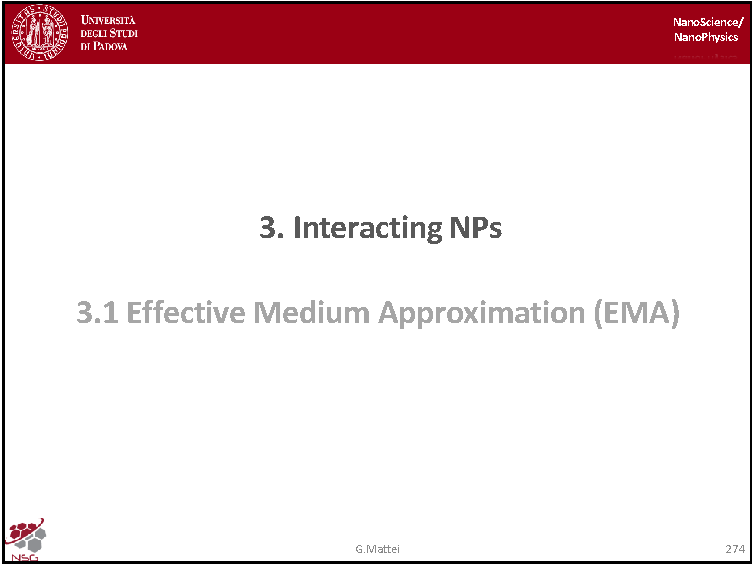
\includegraphics[page=1,width=0.9\textwidth]{../lessons/pdf_file/17_lesson.pdf}
\end{figure}

So far we have seen the properties of nanoparticles systems in which each nanoparticle can be seen as independent, because the inter-particle distance is sufficiently large that the interaction can be safely neglected, in the sense that the external field, that is the plain wave that exits our system is the only excitation each nanoparticle will feel. But, in real world applications, sometimes this approximation is no longer sufficient and we need to see how to deal with situations in which the relative interaction is relevant and how can we use that interaction to obtain better properties out of our systems. So today I would like to show you how to go beyond the non-interacting nanoparticle scheme, which was very successful in producing the Mie theory for spherical nanoparticles in an absorbing medium. The problem is in general very difficult to handle, but under specific assumptions we can quite simplify it in a wide class of interesting materials.
So let us see how we can do that in the \textbf{Effective Medium Approximation class (EMA)}.

\newpage

\subsubsection{Slide 275}

\begin{figure}[h!]
\centering
\includegraphics[page=2,width=0.9\textwidth]{../lessons/pdf_file/17_lesson.pdf}
\end{figure}

The basic idea of Effective Medium Approximation is the following: if we have a system with a matrix whose dielectric function is $\epsilon_{m}$ embedding an array randomly positioned nanoparticles whose dielectric function is $\epsilon$, and nanoparticles are sufficiently small with respect to the wavelenght that we can consider as a dipole. The problem is: can we transform this meta material, that is a material made of different material, in an homogeneous material with an effective dielectric constant $\epsilon_{eff}$.
This is the major question that we have when you want to deal with effective approximation: can we transform an inhomogeneous medium in something which is homogeneous, which is easier to be handled?

There are different schemes of effective medium description for the dielectric function of such a system, but the most successful ones are \textbf{Maxwell-Garnett} approximation (that we will see in details) and \textbf{Brugermann} approximation.

\begin{enumerate}
    \item{Maxwell-Garnett}

    He developed this theory in 1904. He related the effective dielectric function $\epsilon_{eff}$ to the external dielectric function $\epsilon_{m}$ and to the dielectric function of the dipoles $\epsilon$, balanced by the volumetric filling fraction of the dipoles $f$, that is of our nanoparticles.
    If we define the filling fraction $f$ as numerical density of nanoparticles in the system times the volume of the nanpparticles, it can be rewritten as the number of nanoparticles divided by the total volume considered times the volume of the nanoparticles. So this number is between zero and one.

    Of course when $f$ tends to zero, we can safely assume that we are in the independent particle approximation. But which is the threshold at which we need to consider the particles as interacting? (This is the object of today's lesson).

    \item{Brugermann}

    A more symmetric version of this theory is the Brugermann theory. $f$ is the filling fraction corresponding to the phase $\epsilon$, $1-f$ is the filling fraction of phase $\epsilon_{m}$, which is more symmetric expression, while Maxwell-Garnett is more a-symmetric with respect to $f$.
    And so this theory is expected to be more accurate when $f$ is large.
    We will learn what is the meaning of large and small in this contest.

\end{enumerate}

Just to have a final view of all the theories, when we have an effective medium, if we want to compute the optical properties (as the Lamber-Berr expression) we can easily calculate the extinction coefficient ($\gamma$) of the exponential decay of the intensity transversing a given thickness of this homogeneous effective material, where $k_{eff}$ (it is not the wave vector) is the imaginary part of the complex refractive index ($\tilde{n}_{eff}$). $n_{eff}$ is the effective refractive index and $k_{eff}$ is the absorption effective coefficient for that material. Then it is reported the relation between the dielectric function and refractive index:
\begin{equation*}
  \varepsilon _{eff} = \widetilde{n}_{eff}^2
\end{equation*}



\newpage

\subsubsection{Slide 276}

\begin{figure}[h!]
\centering
\includegraphics[page=3,width=0.9\textwidth]{../lessons/pdf_file/17_lesson.pdf}
\end{figure}

Let us see how we can obtain in a simple way the Maxwell-Garnett approximation to deal with a complex system. By the way, We are no longer constrained to have $\epsilon_{m}$ as a purely real quantity: it can be a complex (absorbing) function. So we can go beyond the hypotheses of non absorbing medium.
\begin{enumerate}
    \item{Simple case $\epsilon_{m} = 1$ }
    Starting with the simple case in which we assume for the moment that the external dielectric function is that of vacuum, \( \varepsilon _m =1 \).
     We will see how to renormalize all the equation to handle with a generica value of \( \varepsilon _m \), that can be even complex. The trick is the usual (seen in the classical electrodynamics texktboos). We have an assembly of molecules and we induce a polarization through an electric field, and we need to calculate the effect of the polarization field on the molecule, created by the polarization of all other molecules of the environment. This will produce an additional field which contributes to the local field at the level of the molecule. So that the induced dipole moment $\overline{p}_{loc}$ is usually related through the polarizability to the external field. In this case, the external field is no longer the $\epsilon_{0}$ field (that we send in our system, that is the external field), but it is the local field: that is the external field plus the polarizatin field.

    We have expression for polarization $\overline{P}$ (\( \rho  \) is the concentration of nanoparticles in opur case, but it can be also the concentration of molecules in the system) and local field $\overline{E}_{loc}$ (where the polarization field is easy to be demonstrated).

    The expression for $\overline{E}_{p}$ can be demonstrated with the integral on the right. We draw a sphere around the molecule of the nanoparticle with polarization $\overline{P}$ in the system.
    We want to calculate the additional field (the molecule is on the center of this spherical surface), if there is a polarization in our system \( \va{p} \), we know that we induce on the surface a charge density \( \sigma  \).
    We assume a charge density $\sigma$ on this surface (Polarization projected over the external normal $n$, so locally \( \sigma  \) is related to the projection of \( \va{p} \), which will be in the same direction of the external field projected onto to the normal to the surface). So the contribution of a tinu element of surface \( \dd[]{S}  \) is nothing but \( (-P \cos(\theta ) ) \) (so that we have the projection on the normal). Then we will have the contribution of the field of this charge \( \sigma  \), because if we multiply \( \dd[]{S} \sigma   \) we obtain a \( \dd[]{q}  \) which is an elementary charge of this surface.  So we can calculate the field with the usual expression, which is the charge divided by \( 4 \pi \varepsilon _0 \) and divided by \( r^2 \) (square of the distances from the two charges). So the field produced by the elementary charge (1) on the molecule of the nanoparticle, will be the expressio for \( E_P \). This field will be directed along the normal direction, and for symmetry reason, the resulting field at the molecule level produced by all the elements \( \dd[]{q} \) induced on the surface, will be along the \( P  \) direction of course.
    Ineed, if we consider superior and inferior half sphere the field components perpendicular to $\overline{P}$ will cancel so we can integrate just over the projection of the field of a charge dq over $\overline{P}$ direction (that's why we have an additional $cos \theta$ in the integral).
    $\overline{E}_{p}$ has the same direction of $\overline{P}$.

    Now, we insert $\overline{E}_{loc}$ in the equation for $\overline{P}$ and obtain a self-consistent expression for $\overline{P}$ the polarization as a function of the external field. It contains polarizability $\alpha$ also in the denominator, because we are considering the polarization induced by all the other molecules.
    According to electrodynamics, the polarization should be related to the real external field $\overline{E}_{0}$ through $\chi$ function: which is the effective susceptibility of the first order in linear approximation (we have derived its expression few lessons ago).
    We substitute \( \chi = \varepsilon _{eff} -1  \). In this case we already consider the material as the composed material of the assemble of the molecules as an homogeneous material, so we start to use the effective dielectric function.

    We equate the two expressions for $\overline{P}$ and obtain a self-consistent closed expression for polarizability (it self consistent now, because we consider the system as the effective medium approximation), which is related to the effective dielectric function.
    But now we need to have an explicit expression for $\alpha$ in our system.


\newpage

\subsubsection{Slide 277}

\begin{figure}[h!]
\centering
\includegraphics[page=4,width=0.9\textwidth]{../lessons/pdf_file/17_lesson.pdf}
\end{figure}

    In our case we have spherical nanoparticles in dipolar approximation, than we use polarizability $\alpha$ from Mie theory (we assumed $\epsilon_{m} = 1$, so all $1$ should be multiplied by $\epsilon_{m}$.
    We equate the two equations for $\alpha$ and obtain the explicit result of Maxwell-Garnett (function of two different dielectric functions).
    The two following equation are re-arrangements of this one.

    \item{General case $\epsilon_{m} \neq 1$}
    The general case is more difficult to be derived.
    We must re-normalize $\epsilon{eff}$ and $\epsilon$ and we obtain the fully consistent Maxwell-Garnett derivation with an arbitrary value for $\epsilon_{m}$ (dielectric function of the medium).
    Thus we obtain the fully consistent Maxwell-Garnett derivation with an arbitrary value of the external dielectric function. It is a function of the filling fraction. It is a self-consistent derivation of an homogeneous dielectric function out of a mixing of two different dielectric functions (the one of the nanoparticle and the one of the embedded medium).

\end{enumerate}

 Let us see which can be the effect of this result on the optical properties of a composed material (that is an effective material), or a meta-material, made of a matrix embedding those random assembly of nanoparticles in the dipolar approximation.

\newpage

 \subsubsection{Slide 278}

\begin{figure}[h!]
\centering
\includegraphics[page=5,width=0.9\textwidth]{../lessons/pdf_file/17_lesson.pdf}
\end{figure}

 We can calculate the very same cross-section in Maxwell-Garnett approximation.
 On y-axis we have nothing but the $\gamma$ extinction coefficient (which we saw before and it is a function of the wavelength).
 As a fraction of the filling fraction:
\begin{itemize}
\item  we see that for $f=0.01$. the black curve is practically identical to the results of Mie theory for gold nanoparticles in Silica.
\item The variation with $f=0.1$ is still very small. The difference starts with 20 or 30$\%$.
\item With $f=0.5$ the red-shift is very large.
\end{itemize}
So we can clearly understand that the effect that we have seen, for instance for liquid solution with gold nanoparticle, the concentration will produce a change in the color.
Because, of course, the smaller the concentration, the lower the absorption in the red part of the spectrum and also of the scattering.
So if we look at the extinction, we have an extinction which moves toward the red part of the spectrum.

So, we can easily assume that in the standard RGB division of the color,  we should expect an enhancement of the red component in our system with respect to the others, which are almost unaffected by the interaction (that is the distance between the nanoparticle).
For that reason, we need to expect a colour in solution, which is not due to a change of size, but just a change in relative distance, which is a clear fingerprint of the interaction between the nanoparticles.

As a rule of thumb, up to $10 \%$ of filling fraction $f$ we can still get a very good description of optical properties of our system just using the independent particle approximation, as we did also for ion-implanted nanosystem, in which the relative distance between the nanoparticles was quite low.
When concentration goes above $10 \%$, we need the description of Maxwell-Garnett theory.

In the Maxwell-Garnett theory, there is no explicit reference to the size of the inclusions. This is because we are dealing with volumes which go to zero and radius which goes to zero because we are in dipolar approximation. For that reason, there is a very good agreement of the Maxwell-Garnett with the Mie theory in the dipolar approximation.
Of course, if we need to go beyond the dipolar approximation, the Maxwell-Garnett theory is no longer able to give a correct representation of the effective dielectric function in the system. We need to resort to a more complicated scheme for obtaining an effective medium approximation.

For have a good comparison between Mie theory and Maxwel-Garnett theory:
\begin{itemize}
\item Mie theory: independent particles in anabsorbing medium. Mie was done 1908.
\item Maxwell-Garnett: it goes beyond independent particles, no longer restricted to non-absorbing medium. It was done 1904, so they are independent theories.
\end{itemize}
Consistency check: similar results for these theories.

Of course, when $f$ reaches $0.5$, or when we reach the calculation limit that is the inclusions so densely packed particles that they are a significant fraction of the medium.
The Maxwell-Garnett theory as mentioned is no longer best theory for building the effective Mie theory. The Brugermann theory (which is the most symmetric one) is highly preferable when we have a more balanced fractions of the two phases. But the concept is quite similar.


\newpage

\subsubsection{Slide 279}

\begin{figure}[h!]
\centering
\includegraphics[page=6,width=0.9\textwidth]{../lessons/pdf_file/17_lesson.pdf}
\end{figure}

Now, we want to go beyond the derivation of the simple interaction between dipoles and we want a theory which is able to describe interaction between arbitrarily large nanoparticles. Which changes do we need to introduce to handle with interacting nanoparticles? For instance for the case of multimers.

\newpage

\subsubsection{Slide 280}

\begin{figure}[h!]
\centering
\includegraphics[page=7,width=0.9\textwidth]{../lessons/pdf_file/17_lesson.pdf}
\end{figure}

\begin{itemize}
    \item When dealing with isolated nanoparticle, the polarization of the external field does not play a major role: because in the dipolar approximation an electron can oscillate with any direction with respect to electric field.
    Polarization is basically irrelevant: the situation is symmetric whatever is the relative orientation between the incoming plane wave and the particle, because of the symmetry of the system.

    \item If we break the symmetry introducing another particle (equal to the previous one for example, but it is not a constrate), if we have an external electric field polarized in the longitudinal direction: what can we say about the generale rules to predict where the resonance of this composed system will be with respect to the resonance of the isolated particle?

    The calculation is quite complex, but we can predict where we need to expect the resonance in this case.
    If we assume that we have a longitudinal electric field, the induced dipoles oscillate in the same direction of the polarization. So in the region between the particles we have opposite charges facing each other, forming a depolarization field tending to restore the electronic cloud of dipoles to the static position.

    If we look at the energy of this configuration, we can see that the global energy, when we have opposite charges facing one each other, is the total energy plus the potential energy induced by the interaction between opposite charges (which is negative, because it is an attractive force), so that we have a reduction of the global energy of this configuration (with respect to the kinetic energy of the oscillating electrons plus the potential energy in this case).
    The situation is similar when we have the oscillation on the opposite direction, because for a fixed distance we have this alternation of plus,plus,plus,minus,minus,minus and viceversa.
    So we need to expect that the resonance will shift to lower energy, that is to a longer wavelength when we are in this situation.

    \item On the contrary, with a transverse polarization, the two induced dipoles oscillate in the very same direction, so we have no longer this opposite charges facing, but similar charges facing: so the global energy (apart from the kinetic energy) is increased by the repulsive force between the closer similar induced charges.
    The interaction between opposite charges is no longer high as the one with similar charges, so we need to expect on a very general basis that the global energy of this configuration should be higher with respect to the single independent particle resonance.
    So we need to expect a higher energy resonance with respect to independent particle (lower wavelength).

\end{itemize}

When we have seen ellipsoidal nanoparticles, there was the same effect. When we were in the longitudinal polarization for the ellipsoidal nanoparticle, we have the same situation of the second case. In the ellipsoidal, we can consider that the polarization induces charges that are facing one each other. So they will reduce the energy of the global configuration.

So we can reconduct to the ellipsoidal considering a zero distance between the two nanoparticles in the second case. So this example can be used to explain the resonance of the ellipsoidal nanoparticle.
This is on a very general qualitative base.


\newpage

\subsubsection{Slide 281}

\begin{figure}[h!]
\centering
\includegraphics[page=8,width=0.9\textwidth]{../lessons/pdf_file/17_lesson.pdf}
\end{figure}

We can go beyond this, considering theories for Surface Plasmon Resonance Hybridization.
For instance, we want to calculate where is the resonance of a coassial system in which we have a core made of air inside surrounded by a shell of a metallic material.
People try to obtain results which are very similar to orbitals hybridization in quantum chemistry.

That is, if we have two configurations:
one with a particle, which is nothing but the external configuration and the other one that is a bulk material with a cavity inside, which describes the resonanse inside the core.
We can obtain the core-shell system (that is a metallic shell here (1)) as a hybridization of these two configurations: that is a spherical particle and the cavity resonance:
\begin{itemize}
\item For the particle, from the dipolar approximation, we know that the surface plasmon resonance will occur at the bulk plasmon frequency divided by $\sqrt{3}$, of course assuming vacuum or air as external medium.
\item For the cavity the expression for the resonance of the cavity mode can be easily demonstrated. The resonance of the cavity is the bulk frequency of the metal time \( \sqrt{2/3}  \). This is higher in energy with respect to the sphere.
If we want to build the nanoshell, we need to hybridize this resonance and we get two levels like in the standard Pauli exclusion principle.

\end{itemize}

For each multipolarity, it was calculated the spectral position of this resonance as a function of the two configurations $w_{+}$ and $w_{-}$ (in the left figure) in the nanoshell.
For instance, if we want to predict the dipolar resonance of the semi-shell we can easily calculate it as a function of the ratio of a and b (internal and external radius of the shell) and using $l=1$.
With $a$ going to zero, so we have a closed bulky particle, we need to recover the limiting case of the sphere configuration.
For any intermediate value of the ratio $a/b$ (which goes to 0 to 1), we obtain a continuous evolution of the resonances.

Let us see the plot. In the case of:
\begin{itemize}
    \item{ $\omega_{-}$ (red curve):}
    The frequency goes to zero when $a/b \to 1$, because in this case we have a shell with a negligible thickness.
    With $a/b \to 0$ (a bulk particle), we recover the resonance of the sphere.

    \item{ $\omega_{+}$ (black curve):}
    For $a/b \to 0$ there is the cavity resonance and for $a/b \to 1$ we have a cavity with negligible thickness, which is a bulk material, we recover the bulk value of plasma resonance.

\end{itemize}

This is an effective way to predict the positions of the resonances for complex geometries if we are able to decompose them into simpler geometries and hybridize their corresponding specific resonances. (We will not derive those frequencies, but there is a paper showing it).



\newpage

\subsubsection{Slide 282}

\begin{figure}[h!]
\centering
\includegraphics[page=9,width=0.9\textwidth]{../lessons/pdf_file/17_lesson.pdf}
\end{figure}

We can obtain similar rules for this hybridization scheme for different geometries. If you know the results for the simple case you can obtain hybridization skin which are valid for more complicated situations.

For instance in the case of dimers of equal nanoparticles at distance $d$, we can obtain an hybridization scheme which produces the different expected resonances as a function of the frequency (or energy) of the different configurations in which the two nanoparticles (or their electrons) can oscillate.

The two limiting cases are the very same energy of the resonances, which is if the external medium is vacuum is the $\omega_{p}/\sqrt{3}$, the bulk plasmon divided by the square root of 3, as we have seen.
If we search for the lowest energy configuration, we can use (1) in which we have a symmetric oscillation of charges due to the external polarization field. In this case, we have a lowering of the energy due to the charges facing one each other.

We have already seen the configuration with oscillation in longitudinal direction with respect to external field (second configuration from the top (2)). This is expected to have a higher energy.
But we also have other modes, which can be in principle possible for electronic configurations:
\begin{itemize}
\item (second from the bottom (3)) here we have the oscillation of the two dipoles in anti-phase: polarization in this direction (vertical) but electrons oscillate in a phase different by $\pi$.
\item (first from the top(4)) Here electrons oscillate in transverse direction but with phase opposition.
\end{itemize}
The last two modes are actually not possible to obtain with external polarization:
\begin{itemize}
\item (top mode (4)) because in this case, to induce this oscillation,  if the field is of a wavelength for which the dipolar approximation occurs, there is no chance that the field varies over a space which is of the same size of the nanoparticle, otherwise we would have a multipolar expansion. So that if the field is constant there is no chance to excite with an external field this configuration.
\item (Second from the bottom (3)) Also for the other impossible mode, there is no chance that an homogeneous field excites similiar charges in opposite ways.
\end{itemize}
These modes are called \textbf{Dark Plasmons}: they cannot be excited by external fields. They can be excited but not through photons, but through a localized charge unbalance, that we can produce for instance by shining an electronic beam with a tiny size in between the two nanoparticles (this can be done experimentally), but those are dark plasmons modes in the sense that they can't radiate energy in the far field because they cannot be excited by photons.

In the column on the right we have the expected energy, or frequency, of the resonance in the hybridization scheme which is reported in the paper (on the bottom of the slide): you can obtain a closed evaluation of the dimer interaction as a function of their relative distance (between the particles).

To obtain a very general calculation, which is not based on this hybridization scheme, but if we want to calculate from fundamental properties, or from fully electrodynamics calculations, the expected frequency of dimers, or oligomers or a chain of particles, we need to resort to a bit more complicated theories, like the one in the following calculations.


\newpage

\subsubsection{Slide 283}

\begin{figure}[h!]
\centering
\includegraphics[page=10,width=0.9\textwidth]{../lessons/pdf_file/17_lesson.pdf}
\end{figure}

These calculations are obtained with Generalized Multi-Particles Mie Theory, or GMM approximation. GMM approximation is a generalized version of the Mie theory, but allowing the possibility of having an ensemble of spherical particles (the symmetry of the spherical shape is crucial), they can have different size and can be located at arbitrary distances one from each other. (We will not enter in this theory, because calculation is very difficult, but it is very effective in calculating the resulting local field and far field properties of interacting spherical particles).

I want to show you a couple of examples of the results of this theory.

\begin{itemize}
    \item Example of results of this theory: two silver spherical particle (a silver dimer), we want both far and near field properties.
    Suppose to have a polarization parallel to the dimer axis and we have for instance a diameter $D = 10 nm$ and a gap \( g \) (distance between the two surfaces) which goes from $2 to 5 nm$.
    In the plot there is the extinction cross section of the resulting system with different gaps:

\begin{itemize}
    \item With $G=5 nm$ (same size of the radius) we are basically in independent particle approximation, because the resulting spectrum follows usual Mie theory for single independent particles
    \item If we move particle closer (difficult situation to be obtained experimentally), we see that for a gap which is reduced, we have an hybridization of two resonances: we have a tiny shoulder at higher energies (red dashed in the plot at low $\lambda$) and the main resonance.
    \item With  $G=5 nm$ we develop the two resonances (blue dashed curve): the two bright modes of the resonances, as we have seen in the hybridization scheme. The one with higher $\lambda$ is the one with the field oscillating in the longitudinal direction with respect to the dimer axis.
\end{itemize}

Let us look at the near field distribution:

\begin{itemize}
    \item{left figure: for a gap $g = 5 nm$}.

    The field concentration is in between the gap: because in the region (1) the field is not just the incoherent sum of the two local fields, but there is the interaction field between the facing charges which produces an intense field, or what is called an hot-spot of the electric field (an hot-spot is a place where the field is amplified significantly with respect to external field).

    The color-scale is the local field amplification (field normalized to an external field of $1 V/m$ i.e. the modulus of local field enhancement. In this particular case, we have close to the surface of the particle in the dimers a local field amplification of 32.
    So practically \( \abs{E}  \) is exactly the modulus of the local field enanchement.

    \item {right figure: for a gap $g = 2 nm$}.

    We see that we can go above the single particle resonance, even for silver (we can do better if we are able to obtain particles with a smaller gap).

    Here, in the gap the maximum we reach an amplification of $74$ (two order of magnitude with respect to the external field).
    You may remember that the scattering cross section for surface enhanced ??raman?? scattering is proportional to fourth power of the coefficient of the color-scale; if we round ($74$) up to $100$ we have $10^2$, then it is elevated to the fourth, which is a global amplification of $10^8$ for spectroscopy (a quite remarkable amplification).

\end{itemize}
\end{itemize}


\newpage

\subsubsection{Slide 284}

\begin{figure}[h!]
\centering
\includegraphics[page=11,width=0.9\textwidth]{../lessons/pdf_file/17_lesson.pdf}
\end{figure}

Let us look at other configurations, for instance silver trimers.
In this case, we can expect a larger influence of the polarization. For instance, if we shine light in the direction of $\hat{k}$ vector and electric field polarization is in the direction of the figure, we obtain a cross section (that is a far field property) as in the second plot of above (2), so the resonance is more complicated with respect to the pure single particle or dimer resonances.
If we look at the wavelength with the largest cross section of extinction and we look at the local field, we obtain a local field amplification, which is higher in the gap regions with respect to the trimers and we obtain for the intensity an amplification of $400$ (quite remarkable value).

If we change the polarization direction, as for instance perpendicular to the previous one, we obtain a different configuration, in which we cannot fully exploit the gap amplification. So we have a resonance for the extinction cross-section which goes like that (second plot on the bottom (4)). The local field amplification in this configuration is much lower. You have to choose the best polarization for the system.


\newpage

\subsubsection{Slide 285}

\begin{figure}[h!]
\centering
\includegraphics[page=12,width=0.9\textwidth]{../lessons/pdf_file/17_lesson.pdf}
\end{figure}

To generalize these results, we can think what is the properties of a linear chain of equal sphere nanoparticles. We computed the results for a generalized multiparticle Mie theory and for diamater $D = 10 nm$ and for a dimer. Now the polarization is again along the axis of the chain and we want to see the effect of adding an increasing number of sphere in the chain.

We start with four spheres ($N_s = 4$) (first plot from the top on the right).
In the plot on the left, we see the effect of adding spheres.
The black line has $N_s = 2$ (dimer) with a gap of about $1 nm$.
We go from 2 to 32 nanoparticles: we have a more or less constant position of the first resonance and a movement toward red for the second resonance. This result may be recognized to be similar to having an elongated particle with an aspect ratio which increases.
The situation is almost similar for this polarization of \( N=8 \) (second plot from the bottom on the right).

It is interesting to look at the near field:
\begin{itemize}
\item  for $N_s = 4$, we have an amplification of around $300$;
\item  with $N_s = 8,16$ we do not really get much improvement.
\end{itemize}
This is because the near field amplification is in the gap between two neighbouring nanoparticles.
So the contribution of another nanoparticle to the field is negligible because the local field is supposed to decay as fast as $1/(distance)^3$, so the contribution of additional nanoparticles to the local field in the gap between the two original nanoparticles is expected to be smaller and smaller as a function of the distance. So, of course, we expect an increase because even a tiny contribution should be visible, but not so dramatically.

Hence, the linear chain is a very interesting toy model to understand the rules controlling the local and far field properties of interacting nanosystems.


\newpage

\subsubsection{Slide 286}

\begin{figure}[h!]
\centering
\includegraphics[page=13,width=0.9\textwidth]{../lessons/pdf_file/17_lesson.pdf}
\end{figure}

As a final example I would like to show you a description which generalizes a multiparticle Mie theory of real world application of interacting nanoparticle system and we will focus on the nanoplanet geometry that we already described for the ion beam processing.


\newpage

\subsubsection{Slide 287}

\begin{figure}[h!]
\centering
\includegraphics[page=14,width=0.9\textwidth]{../lessons/pdf_file/17_lesson.pdf}
\end{figure}

In that case, we were interested in the modification of the electromagnetic environment around the nanoparticles to obtain a change in the optical properties both in the near and far field, so that to achieve what is called a \textbf{plasmon tuning}: that is a tuning of the plasma resonance as a function of the processing.

Our aim was to modify the purely spherical nanoparticles, obtained by ion implantation in silica, through an additional treatment in which we ion-irradiate the samples in a controlled way, so that to produce the nanoplanet geometry: that is we modified the core to produce small satellites making an halo around the original planet.
An experimental verification of this is reported in this image (the first on the left below (1)), that is the cross section for unprocessed nanoparticles in silica. If we then add irradiation (Argon irradiation) at $190 keV$, as a function of the flux we are able to produce configuration with an increasing number of satellites, with increasing size and distance with respect to the central nanoplanet. So that we were able to control the geometry of this nanoplanet configuration.

\newpage

\subsubsection{Slide 288}

\begin{figure}[h!]
\centering
\includegraphics[page=15,width=0.9\textwidth]{../lessons/pdf_file/17_lesson.pdf}
\end{figure}

From the optical point of view, we measured the experimental evolution of the extinction cross section for a system in which we irradiate a gold silver nanoclusters alloy, with this composition (\( Au_{0.6} Ag_{0.4} \)), obtaining by sequential ion implantation in silica, and we irradiated with ion with increasing mass in a controlled way as we have described already in the previous slides: from Helium to Neon to Kripton, so that we changed the relative contribution between nuclear and electronic contribution to the energy loss, so that we could tune the transformation of the original nanoparticle into the core satellites objects.

\newpage

\subsubsection{Slide 289}

\begin{figure}[h!]
\centering
\includegraphics[page=16,width=0.9\textwidth]{../lessons/pdf_file/17_lesson.pdf}
\end{figure}

With the generalized multiparticle Mie theory, we obtained a plot for the extinction cross section (right plot, simulation) which nicely reproduces the experimental results as a function of spectra position and shape.

In the Kripton irradiation we have a double-picked resonance which is a clear fingerprint of a neighbouring nanoparticle interaction. Globally, we have a redshift ,as we expect in interacting nano-system.

If we look at how we did this simulation, we basically obtained from the transmissional electron micro graphs an atomistic model of our nanoparticles, then we produced different configuration and we simulated with the GMM theory the far field properties.


\newpage

\subsubsection{Slide 290}

\begin{figure}[h!]
\centering
\includegraphics[page=17,width=0.9\textwidth]{../lessons/pdf_file/17_lesson.pdf}
\end{figure}

Of course we obtained also a near field calculation. That is: from the structure (left (1)) we created this model (on the left, figure (2)) (with an average satellite size with respect to the original planet) and we were able to calculate for instance in plane (which is a section of this 3D configuration) the local field enhancement. We see that there were hot-spots of electric field in the gap regions between satellites and original core. As we have seen in the figure (left (3)): there is a local field amplification of around $20$ (in terms of the local field enanchement)

In the case of Kripton irradiation (on the right): we see that the original nanoparticles were so heavily modified by the very energetic Kripton ions, that the resulting configuration in now made of satellites of the very same size of the resulting central planet. So in that case we have even larger amplification of the field, with respect of the previous configuration, of course in the gap between two neighbours nanoparticles like in this case (figure (6)).

The message is: if you are able to modify the local environment around the nanoparticle, you are able to produce local field hot-spots, which produces an amplification of the local field at at least one order of magnitude, or even more by tuning the level of interaction.
This has a lot of ??biproduca?? applications. For instance, in this kind of system we investigated intensively for the non linear optical properties, as we will see in the following, but for the moment we are looking at the linear properties.


\newpage

\subsubsection{Slide 291}

\begin{figure}[h!]
\centering
\includegraphics[page=18,width=0.9\textwidth]{../lessons/pdf_file/17_lesson.pdf}
\end{figure}

Let us look at the local field of a given configuration in the GMM theory by comparing two situations, in which we have the effect of the composition into play.

We would like to compare an alloy gold and siver with respect to pure silver nanostructure.  The result is reported here.
This is the configuration that we chose (fig (1)). For the two situations we just changed the composition of the nanoplanets and the original particles inside.


\begin{itemize}
\item The plane is initially below with respect to the central figure.

In these two pictures, I reported the local field calculated on a plane reported in the central figure, which is the cross section of the configuration near the south pole of the original planet.

For the golden silver alloy (left figure) we have a slightly lower field amplification with respect to the pure silver (right figure), because we are still close to the inter-band transition of gold, which depresses the global intensity of the near field.
Of course, silver is a better plasmonic metal with respect to gold or gold silver in this case.


\item Plane closer to the equatorial plane in the central figure.

If we change the plane in which we calculate the local field, in this new plane which is closer to the equatorial plane, we have a still higher field amplification.


\item Equatorial plane.

When we reach the equatorial plane we obtain an amplification which is around $67$ in the case of silver in this tiny hot-spot and $17$ in the case of the alloy. So you can think what is exactly the effect of the composition in this particular case.

\item Plane goes above the equatorial plane.

Then, if we move the plane in this tomographic view of the local field away from the equatorial plane, and we move closer to the north pole, the local field amplification starts to decrease and we recover more or less the same situation as before.

\end{itemize}


But this is a sort of statistical situation, because it depends on how many gaps between two neighbouring nanoparticles we are sampling in that peculiar plane, so that statistically we can obtain a local field enhancement at each latitude, so that there is no particular restriction on that.
It depends just of course on the polarization, of course when \( \va{k} \) is moving toward the north pole to the south of the system and we are looking at a polarization that is in the horizontal direction, of course the largest chances to have an hot-spot is on the equatorial plane.



\clearpage


\end{document}
